%%%%%%%%%%%%%%%%%%%%%%%%%%%%%%%%%%%%%%%%%%%%%%%%%%%%%%%%%%%%%%%%%%%%%%%%%%%%%%%%
% CSC2059 Practical 4
%%%%%%%%%%%%%%%%%%%%%%%%%%%%%%%%%%%%%%%%%%%%%%%%%%%%%%%%%%%%%%%%%%%%%%%%%%%%%%%%

\documentclass{csc2059practical}

\setpracticalnumber{4}

\setpracticaltitle{Classes, Resource Management and Stacks}

\setpracticalsubtitle{From Objects to Abstract Data Types}

\setpracticalauthor{
Dr Giuseppe Trombino\\
School of Electronics, Electrical Engineering and Computer Science\\
Queen's University Belfast
}
\setpracticaldate{}


\begin{document}

\maketitle

\tableofcontents
\clearpage

%%%%%%%%%%%%%%%%%%%%%%%%%%%%%%%%%%%%%%%%%%%%%%%%%%%%%%%%%%%%%%%%%%%%%%%%%%%%%%%%
% Introduction
%%%%%%%%%%%%%%%%%%%%%%%%%%%%%%%%%%%%%%%%%%%%%%%%%%%%%%%%%%%%%%%%%%%%%%%%%%%%%%%%

\frontsection{Introduction}

In previous practicals you have explored the foundations of C++ programming,
including compilation, Makefiles, pointers, and manual memory management.

This practical brings these ideas together through the use of classes and
abstract data types.

You will begin by examining and using an existing class, before implementing
your own class that manages dynamically allocated memory. You will then extend
an existing stack implementation and finally use stacks as abstractions for
solving algorithmic problems.

The emphasis throughout this practical is on developing an understanding of
ownership, abstraction, and code reuse.

%%%%%%%%%%%%%%%%%%%%%%%%%%%%%%%%%%%%%%%%%%%%%%%%%%%%%%%%%%%%%%%%%%%%%%%%%%%%%%%%
% Learning Outcomes
%%%%%%%%%%%%%%%%%%%%%%%%%%%%%%%%%%%%%%%%%%%%%%%%%%%%%%%%%%%%%%%%%%%%%%%%%%%%%%%%

\begin{learningoutcomes}

By the end of this practical, you should be able to:

\begin{itemize}

\item Read and use existing C++ classes.

\item Implement constructors, destructors and copy constructors.

\item Develop classes that manage dynamically allocated resources.

\item Extend an existing abstract data type implementation.

\item Use a stack abstraction to solve simple algorithmic problems.

\item Apply testing and demonstrations to guide implementation decisions.

\end{itemize}

\end{learningoutcomes}

%%%%%%%%%%%%%%%%%%%%%%%%%%%%%%%%%%%%%%%%%%%%%%%%%%%%%%%%%%%%%%%%%%%%%%%%%%%%%%%%
% Time estimation
%%%%%%%%%%%%%%%%%%%%%%%%%%%%%%%%%%%%%%%%%%%%%%%%%%%%%%%%%%%%%%%%%%%%%%%%%%%%%%%%

\begin{infobox}{Estimated Effort}

This practical has been designed for a two-hour session.

\end{infobox}
%%%%%%%%%%%%%%%%%%%%%%%%%%%%%%%%%%%%%%%%%%%%%%%%%%%%%%%%%%%%%%%%%%%%%%%%%%%%%%%%
% Before You Begin
%%%%%%%%%%%%%%%%%%%%%%%%%%%%%%%%%%%%%%%%%%%%%%%%%%%%%%%%%%%%%%%%%%%%%%%%%%%%%%%%


\frontsection{Before You Begin}

Before starting this practical, take a moment to check your understanding of
the following topics.

You do not need to be an expert in every area, but you should recognise most
of these concepts and know where you have encountered them previously.

\begin{itemize}

\item I can declare and initialise objects.

\item I can create objects dynamically using \texttt{new}.

\item I can release dynamically allocated memory using
\texttt{delete}.

\item I can distinguish between stack and heap allocation.

\item I can separate declarations (\texttt{.h}) from
implementations (\texttt{.cpp}).

\item I can compile programs using a Makefile.

\item I know how to execute demonstrations and tests contained
within a repository.

\item I can explain the purpose of constructors and destructors.

\item I can describe what a copy constructor does.

\item I can explain the behaviour of a stack data structure.

\end{itemize}

If several items feel unfamiliar, consider revisiting:

\begin{itemize}

\item Practical 2 --- Functions, Compilation and Makefiles

\item Practical 3 --- Pointers and Manual Memory Management

\end{itemize}

%%%%%%%%%%%%%%%%%%%%%%%%%%%%%%%%%%%%%%%%%%%%%%%%%%%%%%%%%%%%%%%%%%%%%%%%%%%%%%%%
% Repository Access
%%%%%%%%%%%%%%%%%%%%%%%%%%%%%%%%%%%%%%%%%%%%%%%%%%%%%%%%%%%%%%%%%%%%%%%%%%%%%%%%

\frontsection{Repository Access}

Access the Practical 4 repository from Canvas and clone it to your local
machine.

Before beginning the exercises:

\begin{itemize}

\item ensure the repository compiles successfully;

\item explore the available demonstrations;

\item execute the provided tests;

\item familiarise yourself with the repository structure.

\end{itemize}

Throughout this practical, demonstrations and tests are intended to guide your
implementation decisions and provide feedback on your progress.

\begin{figure}[htbp]
\centering
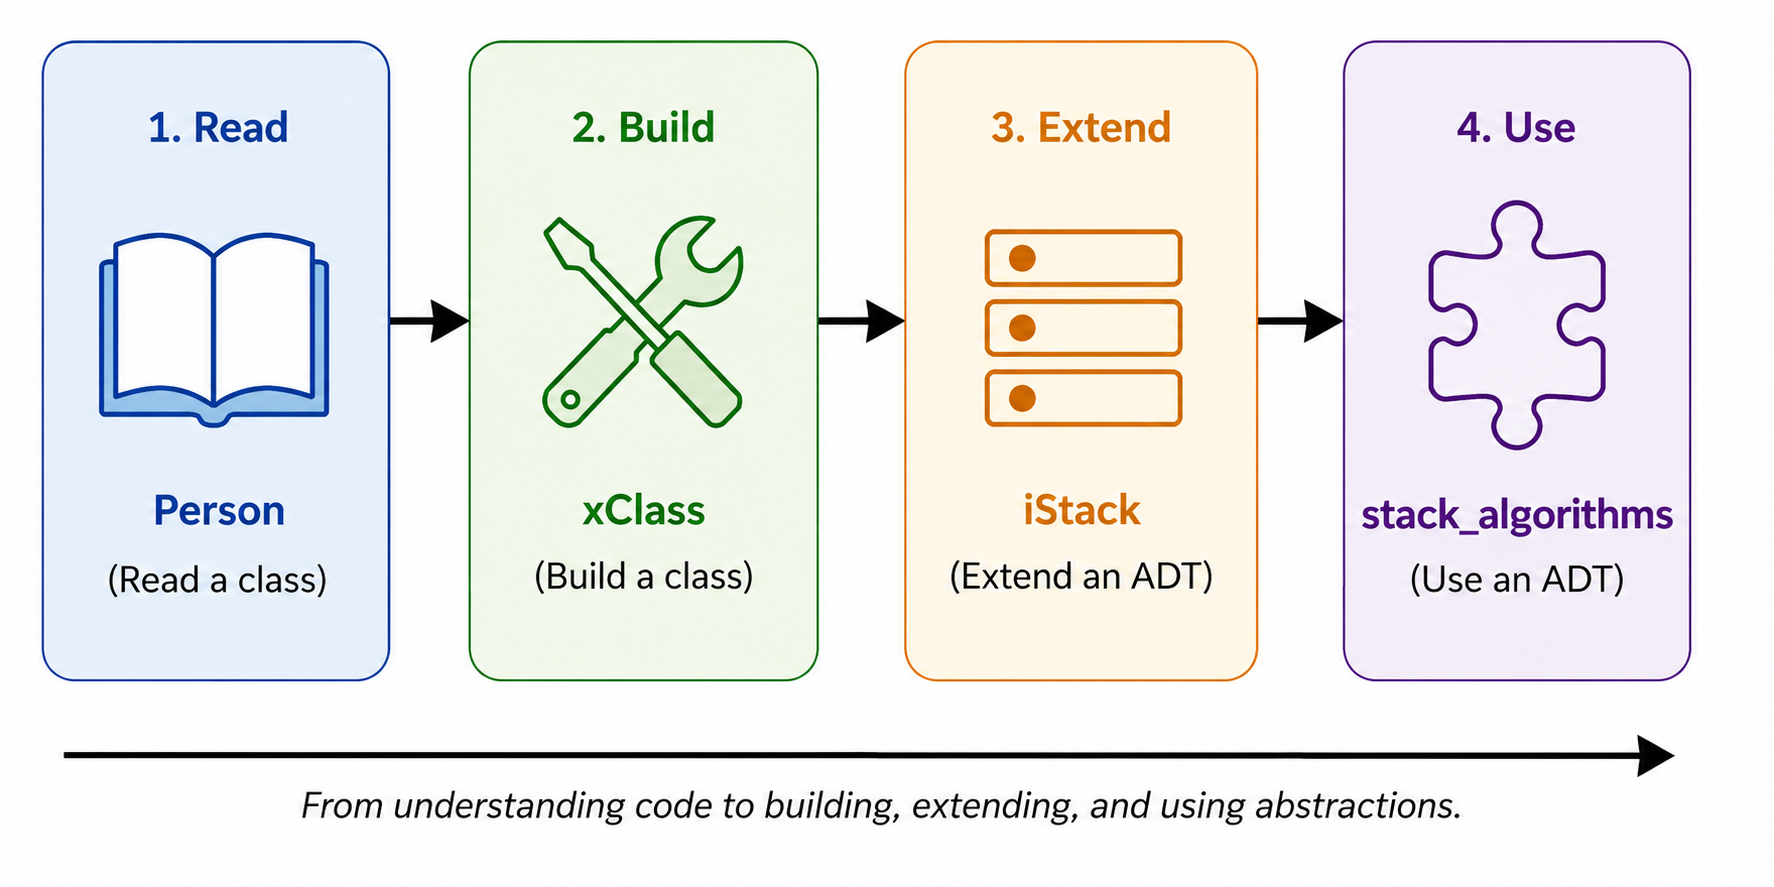
\includegraphics[width=0.85\textwidth]{../../../assets/figures/practical04/Figure01.png}
\label{fig:PracticalProgression}
\caption{Practical Progression Overview}
\end{figure}


%%%%%%%%%%%%%%%%%%%%%%%%%%%%%%%%%%%%%%%%%%%%%%%%%%%%%%%%%%%%%%%%%%%%%%%%%%%%%%%%
% Repository Tour
%%%%%%%%%%%%%%%%%%%%%%%%%%%%%%%%%%%%%%%%%%%%%%%%%%%%%%%%%%%%%%%%%%%%%%%%%%%%%%%%

\frontsection{Repository Tour}

The repository is organised around four core activities.

\begin{center}

\begin{tabular}{ll}

\textbf{Component} & \textbf{Purpose}\\
\hline

\texttt{Person} &
Reading and using existing classes \\

\texttt{xClass} &
Building a resource-owning class \\

\texttt{iStack} &
Extending an abstract data type \\

\texttt{stack\_algorithms} &
Using an abstract data type \\

\texttt{examples} &
Demonstrations and experimentation \\

\texttt{tests} &
Guided implementation support \\

\end{tabular}

\end{center}


By the end of this practical, you will have progressed from reading existing
classes, to building your own, to extending and using abstract data types.

%%%%%%%%%%%%%%%%%%%%%%%%%%%%%%%%%%%%%%%%%%%%%%%%%%%%%%%%%%%%%%%%%%%%%%%%%%%%%%%%
% Section 1 starts here
%%%%%%%%%%%%%%%%%%%%%%%%%%%%%%%%%%%%%%%%%%%%%%%%%%%%%%%%%%%%%%%%%%%%%%%%%%%%%%%%

%%%%%%%%%%%%%%%%%%%%%%%%%%%%%%%%%%%%%%%%%%%%%%%%%%%%%%%%%%%%%%%%%%%%%%%%%%%%%%%%
\section{Reading and Using Existing Classes}
%%%%%%%%%%%%%%%%%%%%%%%%%%%%%%%%%%%%%%%%%%%%%%%%%%%%%%%%%%%%%%%%%%%%%%%%%%%%%%%%

\begin{infobox}{Estimated Effort}

    Approximate completion time: 10--15 minutes.
    
\end{infobox}

\begin{learningoutcomes}
    In this section you will:
\begin{itemize}
    
    \item explore an existing C++ class;
    
    \item identify common class components such as constructors,
    destructors and accessor functions;
    
    \item create and manipulate objects;
    
    \item distinguish between objects allocated on the stack and objects
    allocated dynamically.
\end{itemize}


\end{learningoutcomes}

The repository provides a complete implementation of the
\texttt{Person} class. Your goal is not to modify this class, but to
become familiar with its structure and how it is used.

The implementation consists of:

\begin{itemize}

\item \texttt{include/Person.h}

\item \texttt{src/Person.cpp}

\item \texttt{examples/demo\_person.cpp}

\item \texttt{tests/test\_person.cpp}

\end{itemize}

Begin by examining \texttt{Person.h}.

Identify the following components:

\begin{itemize}

\item parameterised constructor;

\item default constructor;

\item getter functions;

\item setter functions;

\item overloaded equality operator;

\item private data members.

\end{itemize}

Notice that some member functions have the keyword
\texttt{const} appended to their declaration.

This indicates that the function does not modify the state of the
object.

For example:

\begin{cppcode}
std::string get_given_name() const;
\end{cppcode}

promises that calling the function will not change the stored
attributes of the \texttt{Person} object.

\subsection*{Running the Demonstration}

Execute the demonstration program.

\begin{terminal}
make demo-person
\end{terminal}

Observe the output produced.

Consider the following questions:

\begin{itemize}

\item How are objects created?

\item How are member functions invoked?

\item How does dynamic allocation differ from ordinary object creation?

\item What role does \texttt{delete} play in the example?

\end{itemize}

\subsection*{Running the Tests}

Execute the provided tests.

\begin{terminal}
make test-person
\end{terminal}

All tests should pass successfully.

Unlike later sections of this practical, you are not expected to
modify the \texttt{Person} implementation.

Instead, this section provides an opportunity to read existing code,
understand its structure, and become familiar with common C++ class
constructs.

\begin{tipbox}

Reading code written by others is an important programming skill.

As software systems become larger, developers spend a significant
amount of time understanding existing implementations before adding
new functionality.

\end{tipbox}

\begin{reflectionbox}

How does the \texttt{Person} class differ from the programs developed
in previous practicals?

Which aspects of the implementation already feel familiar, and which
features are new to you?

\end{reflectionbox}

%%%%%%%%%%%%%%%%%%%%%%%%%%%%%%%%%%%%%%%%%%%%%%%%%%%%%%%%%%%%%%%%%%%%%%%%%%%%%%%%
\section{Building a Resource-Owning Class}
%%%%%%%%%%%%%%%%%%%%%%%%%%%%%%%%%%%%%%%%%%%%%%%%%%%%%%%%%%%%%%%%%%%%%%%%%%%%%%%%

\begin{infobox}{Estimated Effort}
Approximate completion time: 25--30 minutes.
\end{infobox}

\begin{learningoutcomes}
    In this section you will:
\begin{itemize}

    
    \item implement constructors and destructors;
    \item manage dynamically allocated memory safely;
    \item implement copy semantics;
    \item interpret test feedback to guide development;
    \item practise incremental implementation.
\end{itemize}
\end{learningoutcomes}

In this section you will implement parts of the
\texttt{xClass} implementation.

Unlike the \texttt{Person} class explored previously,
\texttt{xClass} owns dynamically allocated memory.

Correct resource management is therefore essential to avoid memory leaks,
invalid accesses and unintended sharing of resources.

\subsection*{Repository Files}

This exercise focuses on the following files.

\begin{itemize}

\item \texttt{include/xClass.h}

\item \texttt{src/xClass.cpp}

\item \texttt{examples/demo\_xclass.cpp}

\item \texttt{tests/test\_xclass.cpp}

\end{itemize}

\subsection*{Running the Tests}

Execute the tests for this section.

\begin{terminal}
make test-xclass
\end{terminal}

At this stage, several tests should fail.

This is expected.

Your goal is to implement the missing functionality incrementally until
all tests pass.

\subsection*{Suggested Implementation Order}

To avoid becoming overwhelmed, implement the member functions in the
following order.

\begin{enumerate}

\item Constructor

\item \texttt{print\_data()}

\item \texttt{data\_at()}

\item \texttt{ave\_data()}

\item \texttt{range\_data()}

\item Destructor

\item Copy constructor

\item \texttt{operator+=}

\end{enumerate}

\subsection*{Constructor}

Begin by implementing the constructor.

The class stores two pieces of information:

\begin{itemize}

\item the number of elements;

\item a dynamically allocated array.

\end{itemize}

You will need to allocate sufficient memory to store all values.

For example:

\begin{cppcode}
data = new int[size];
\end{cppcode}

Once memory has been allocated, initialise the elements appropriately.

\begin{tipbox}

Large programming tasks become easier when broken into smaller
components.

Implement one function, rerun the tests, and then move on to the next
objective.

\end{tipbox}

After implementing the constructor, rerun the tests.

\begin{terminal}
make test-xclass
\end{terminal}

Observe which tests now pass before continuing.

\subsection*{Accessor Functions}

Several member functions provide access to the stored information.

Implement:

\begin{itemize}

\item \texttt{length()}

\item \texttt{data\_at()}

\item \texttt{ave\_data()}

\item \texttt{range\_data()}

\end{itemize}

Pay particular attention to boundary conditions.

Consider how your implementation should behave if an invalid index is
supplied.

Once these functions are implemented, rerun the tests.

\begin{terminal}
make test-xclass
\end{terminal}

Notice how incremental improvements reduce the number of failing tests.

\subsection*{Destructor}

Objects that allocate memory dynamically are also responsible for
releasing it.

The destructor should deallocate any memory owned by the object.

\begin{cppcode}
delete[] data;
\end{cppcode}

Failure to release dynamically allocated memory can lead to memory
leaks.

Execute the tests again before moving forward.

\begin{terminal}
make test-xclass
\end{terminal}

\subsection*{Copy Constructor}

Copying an object that owns memory requires more care than copying
ordinary variables.

Simply copying the pointer value causes two objects to reference the
same memory location.

\begin{figure}[htbp]
\centering
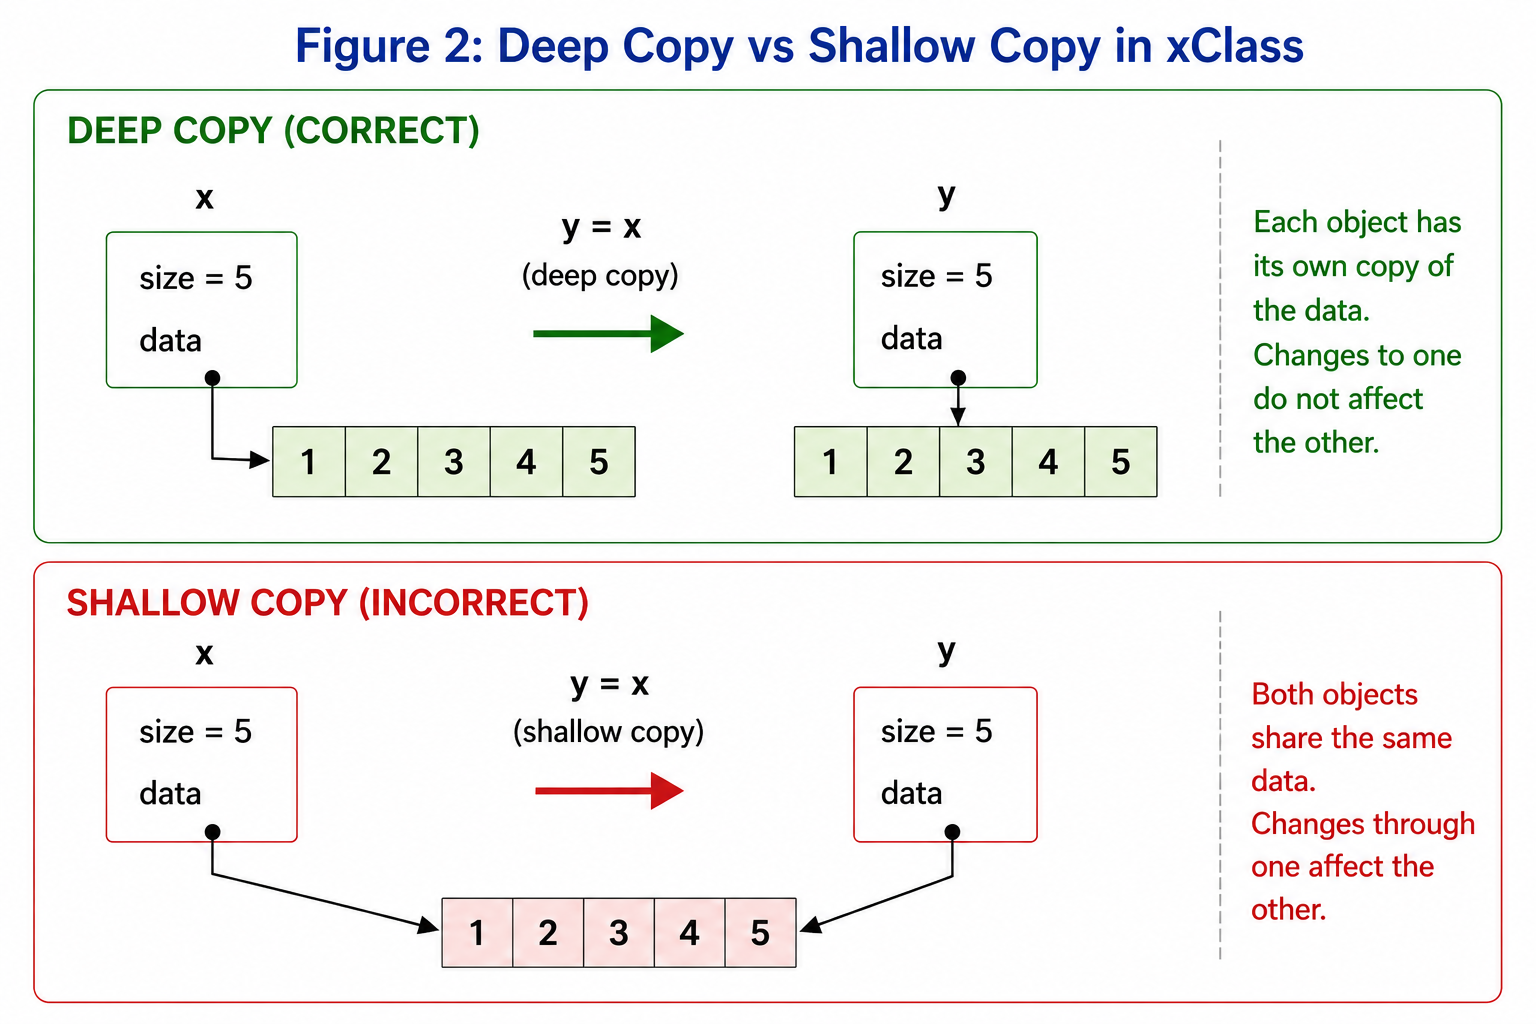
\includegraphics[width=0.85\textwidth]{../../../assets/figures/practical04/Figure02.png}
\label{fig:deepVsshallowCopy}
\caption{Deep copy vs Shallow Copy in xClass}
\end{figure}

Instead, a new array should be allocated and the stored values copied
individually.

\begin{cppcode}
for (int i = 0; i < size; i++)
{
    // copy one element at a time
}
\end{cppcode}

Once your copy constructor is complete, rerun the tests.

\begin{terminal}
make test-xclass
\end{terminal}

\subsection*{Operator Overloading}

The overloaded \texttt{operator+=} combines the contents of two objects.

The resulting object should contain all values stored in both operands.

Think carefully about:

\begin{itemize}

\item how much memory is required;

\item preserving existing values;

\item updating the stored size.

\end{itemize}

Run the tests one final time.

\begin{terminal}
make test-xclass
\end{terminal}

Aim for all tests to pass before moving to the next section.

\subsection*{Running the Demonstration}

Execute:

\begin{terminal}
make demo-xclass
\end{terminal}

Observe how the output evolves as your implementation becomes more
complete.

\begin{commonerror}

Using ordinary assignment on pointers copies addresses rather than
data.

If two objects share the same dynamically allocated array, unexpected
behaviour may occur.

\end{commonerror}

\begin{reflectionbox}

Why is a copy constructor necessary for classes that manage dynamically
allocated memory?

How would the behaviour differ if only the pointer value were copied?

\end{reflectionbox}

%%%%%%%%%%%%%%%%%%%%%%%%%%%%%%%%%%%%%%%%%%%%%%%%%%%%%%%%%%%%%%%%%%%%%%%%%%%%%%%%
\section{Extending a Stack ADT}
%%%%%%%%%%%%%%%%%%%%%%%%%%%%%%%%%%%%%%%%%%%%%%%%%%%%%%%%%%%%%%%%%%%%%%%%%%%%%%%%

\begin{infobox}{Estimated Effort}
Approximate completion time: 30 minutes.
\end{infobox}

\begin{learningoutcomes}

\begin{itemize}

\item extend an existing abstract data type;

\item implement additional stack operations;

\item preserve the behaviour of an existing data structure;

\item reason about invariants;

\item use public tests to validate implementations.

\end{itemize}

\end{learningoutcomes}

In previous practicals, you have implemented data structures from
scratch.

In this section, you will work from an existing implementation.

This is a common software engineering activity. Developers frequently
need to understand existing code bases before extending their
functionality.

\subsection*{Repository Files}

This exercise focuses on:

\begin{itemize}

\item \texttt{include/iStack.h}

\item \texttt{include/iStackNode.h}

\item \texttt{src/iStack.cpp}

\item \texttt{src/iStackNode.cpp}

\item \texttt{examples/demo\_stack\_extension.cpp}

\item \texttt{tests/test\_stack\_extension.cpp}

\end{itemize}

Begin by reading the existing implementation.

Identify:

\begin{itemize}

\item how nodes are represented;

\item how values are pushed onto the stack;

\item how values are removed;

\item how the stack keeps track of its contents.

\end{itemize}

\subsection*{Running the Tests}

Execute the tests for this section.

\begin{terminal}
make test-stack-extension
\end{terminal}

At this stage, all tests should fail.

This is expected.

Your goal is to extend the existing implementation by completing two
member functions.

\begin{figure}[htbp]
\centering
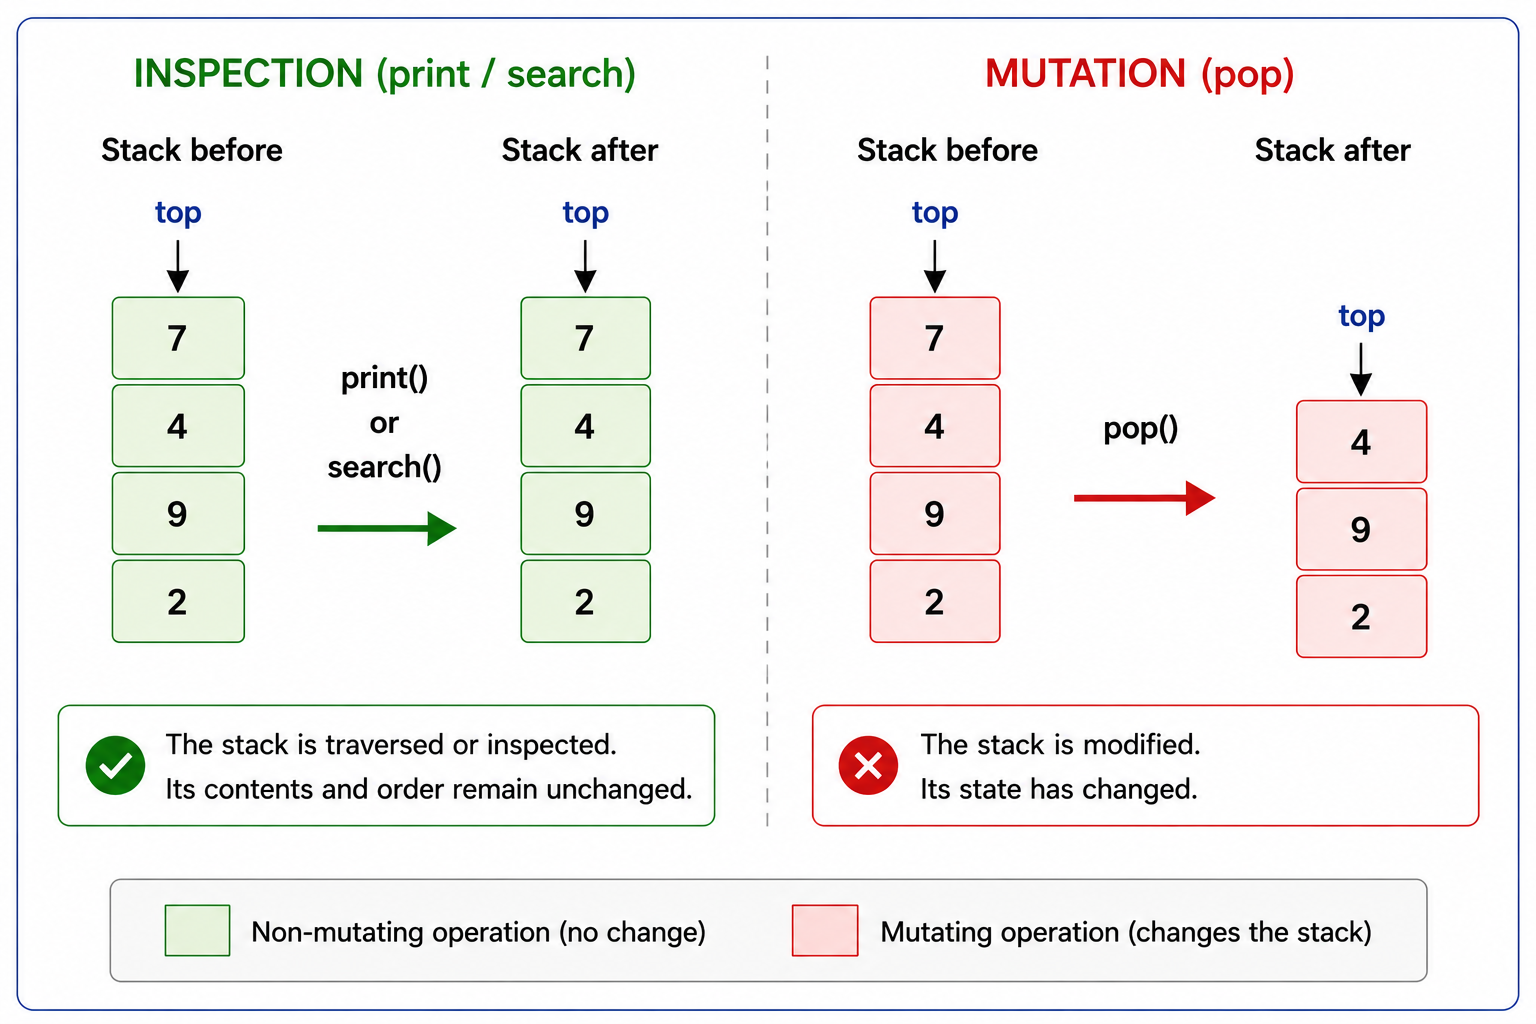
\includegraphics[width=0.85\textwidth]{../../../assets/figures/practical04/Figure03.png}
\label{fig:TraversalWoModification}
\caption{Traversal without Modification}
\end{figure}

\subsection*{Printing the Stack}

Implement the \texttt{print()} member function.

The function should display the contents of the stack without modifying
its state.

Think carefully about how traversal differs from removal.

The stack should contain exactly the same values before and after the
operation.

Once implemented, rerun the tests.

\begin{terminal}
make test-stack-extension
\end{terminal}

Observe which tests now pass.

\subsection*{Searching the Stack}

Implement the \texttt{search()} member function.

The function should locate a given value and return its position within
the stack.

Consider the following questions.

\begin{itemize}

\item How should an empty stack behave?

\item What should happen if the value is not present?

\item Should the search operation modify the stack?

\end{itemize}

After implementing the function, rerun the tests.

\begin{terminal}
make test-stack-extension
\end{terminal}

Aim to pass all tests before continuing.

\clearpage

\begin{tipbox}

When extending an existing data structure, it is important to preserve
its original behaviour.

Adding new functionality should not introduce unintended side effects.

\end{tipbox}

\subsection*{Running the Demonstration}

Execute:

\begin{terminal}
make demo-stack-extension
\end{terminal}

Observe the behaviour of the stack before and after calling
\texttt{search()} and \texttt{print()}.

The contents of the stack should remain unchanged.

\begin{commonerror}

Removing elements while traversing a stack changes its state.

Operations such as \texttt{print()} and \texttt{search()} should
inspect the stack rather than consume it.

\end{commonerror}

\begin{reflectionbox}

Why might preserving the state of a stack be important?

Can you think of situations where modifying a data structure during
inspection would cause problems?

\end{reflectionbox}


%%%%%%%%%%%%%%%%%%%%%%%%%%%%%%%%%%%%%%%%%%%%%%%%%%%%%%%%%%%%%%%%%%%%%%%%%%%%%%%%
\section{Using a Stack as an Abstraction}
%%%%%%%%%%%%%%%%%%%%%%%%%%%%%%%%%%%%%%%%%%%%%%%%%%%%%%%%%%%%%%%%%%%%%%%%%%%%%%%%

\begin{infobox}{Estimated Effort}
Approximate completion time: 30--35 minutes.
\end{infobox}

\begin{learningoutcomes}

\begin{itemize}

\item use an existing abstract data type to solve problems;

\item distinguish between extending and using a data structure;

\item implement algorithms using only a public interface;

\item reason about algorithmic constraints;

\item develop reusable components.

\end{itemize}

\end{learningoutcomes}

In the previous section, you extended an existing stack
implementation.

In this section, you will take on a different role.

Rather than modifying the stack itself, you will use the stack as a
tool for solving problems.

This distinction is important.

Sometimes we design data structures.

At other times, we use them as building blocks for larger systems.



\subsection*{Repository Files}

This exercise focuses on:

\begin{itemize}
    
    \item \texttt{include/stack\_algorithms.h}
    
    \item \texttt{src/stack\_algorithms.cpp}
    
    \item \texttt{examples/demo\_stack\_algorithms.cpp}
    
    \item \texttt{tests/test\_stack\_algorithms.cpp}
    
\end{itemize}

\begin{figure}[htbp]
\centering
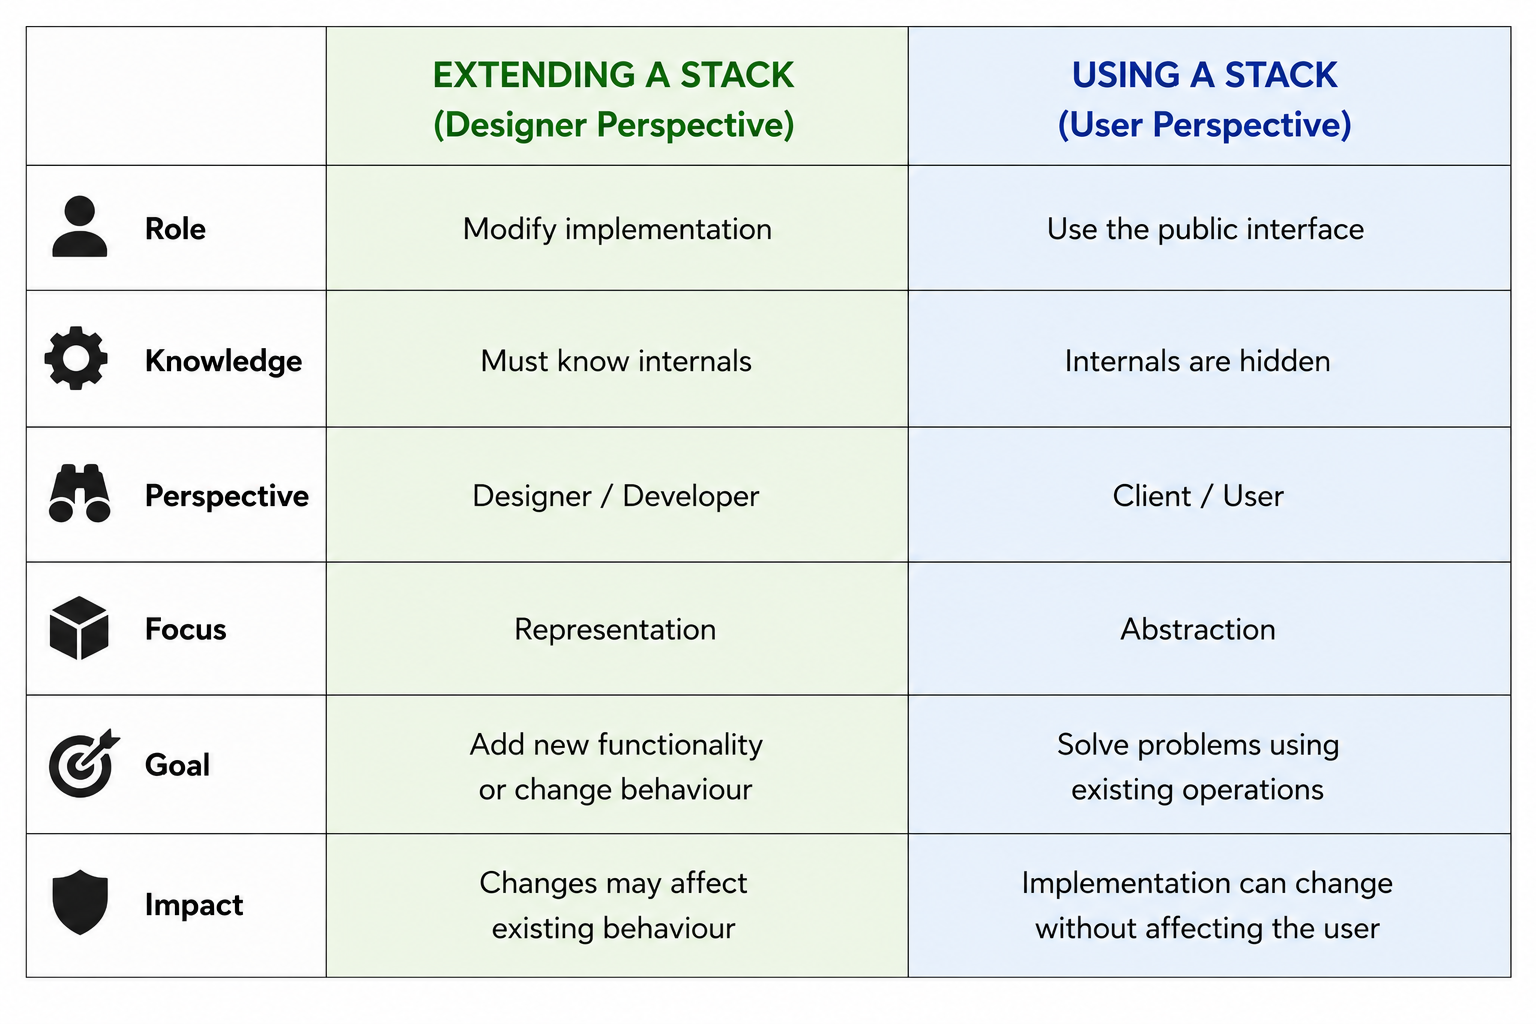
\includegraphics[width=0.85\textwidth]{../../../assets/figures/practical04/Figure04.png}
\label{fig:ExtendingVsUsing}
\caption{Extending vs using an Abstract Data Type}
\end{figure}


Unlike the previous section, you should treat the stack
implementation as complete.

Only its public interface should be used.

\subsection*{Running the Tests}

Execute:

\begin{terminal}
make test-stack-algorithms
\end{terminal}

Initially, several tests should fail.

Your objective is to implement each algorithm incrementally until all
tests pass.

\subsection*{Searching a Stack}

Implement the function:

\begin{cppcode}
int search_stack(iStack& s, int value);
\end{cppcode}

This function performs a similar task to the member function developed
in the previous section.

However, this time the implementation must rely exclusively on the
stack's public interface.

Consider the following questions.

\begin{itemize}

\item Which operations are available?

\item Can the stack be traversed directly?

\item How can temporary storage be used to preserve the original stack?

\end{itemize}

Once implemented, rerun the tests.

\begin{terminal}
make test-stack-algorithms
\end{terminal}

\subsection*{Reversing a Stack}

Implement:

\begin{cppcode}
void reverse_stack(iStack& source,
                   iStack& destination);
\end{cppcode}

The function should transfer values from one stack to another while
reversing their order.

Think carefully about what happens when values are repeatedly removed
from the top of a stack.

After implementation, rerun the tests.

\begin{terminal}
make test-stack-algorithms
\end{terminal}

\subsection*{Removing from the Bottom}

Implement:

\begin{cppcode}
bool remove_from_bottom(iStack& s,
                        int index);
\end{cppcode}

Unlike ordinary stack operations, this function requires access to an
element that is not immediately available.

You may find it useful to consider how temporary storage can be used
to reach deeper elements while preserving the overall structure.

Run the tests again before continuing.

\begin{terminal}
make test-stack-algorithms
\end{terminal}

\begin{tipbox}

Abstract data types are valuable because they hide implementation
details.

By relying only on a public interface, algorithms become easier to
reuse and maintain.

\end{tipbox}

\subsection*{Running the Demonstration}

Execute:

\begin{terminal}
make demo-stack-algorithms
\end{terminal}

Observe how the stack can be manipulated without requiring knowledge
of its internal representation.

Notice that the same implementation would still work even if the stack
were redesigned internally.

\begin{commonerror}

Attempting to access internal node pointers defeats the purpose of
using an abstract data type.

Algorithms should interact with the stack through its public
operations only.

\end{commonerror}

\begin{reflectionbox}

How does using an abstract data type differ from extending one?

What advantages are gained by relying only on a public interface?

\end{reflectionbox}

%%%%%%%%%%%%%%%%%%%%%%%%%%%%%%%%%%%%%%%%%%%%%%%%%%%%%%%%%%%%%%%%%%%%%%%%%%%%%%%%
\section{Fast Finisher Challenges}
%%%%%%%%%%%%%%%%%%%%%%%%%%%%%%%%%%%%%%%%%%%%%%%%%%%%%%%%%%%%%%%%%%%%%%%%%%%%%%%%

\begin{challengebox}

The following activities are entirely optional.

They are intended for students who complete the core practical early
and would like to explore additional ideas.


\end{challengebox}

\subsection*{Challenge 1: Defensive Programming}

Several functions within \texttt{xClass} assume valid inputs.

Consider improving the robustness of the implementation.

Examples include:

\begin{itemize}
    
    \item preventing negative sizes;
    
    \item checking bounds in \texttt{data\_at()};
    
    \item handling empty arrays in \texttt{ave\_data()};
    
    \item deciding how invalid operations should behave.
    
\end{itemize}

How should a well-designed class respond when it is used incorrectly?

If you want to tackle these, we have prepared some tests that can guide you through the challenges.  You can run these with

\begin{terminal}
    make test-xclass-challenge
\end{terminal}


\subsection*{Challenge 2: Robust Stack Algorithms}

Can your stack algorithms cope with unusual situations?

Investigate behaviour when:

\begin{itemize}

\item the stack is empty;

\item a search target is not present;

\item an invalid index is supplied to
\texttt{remove\_from\_bottom()}.

\end{itemize}

Are there opportunities to simplify or improve your implementation?

\subsection*{Challenge 3: Reversing User Input}

Create a small program that repeatedly accepts integer values from the
user until a sentinel value is entered.

Store the values in a stack and then display them in reverse order.

For example:

\begin{terminal}
Input:

5
8
13
21
*

Output:

21 13 8 5
\end{terminal}

This activity demonstrates one of the classical applications of stack
data structures.


%%%%%%%%%%%%%%%%%%%%%%%%%%%%%%%%%%%%%%%%%%%%%%%%%%%%%%%%%%%%%%%%%%%%%%%%%%%%%%%%
\frontsection{Reflection}
%%%%%%%%%%%%%%%%%%%%%%%%%%%%%%%%%%%%%%%%%%%%%%%%%%%%%%%%%%%%%%%%%%%%%%%%%%%%%%%%

Consider the following questions.

\begin{itemize}

\item Which concepts from previous practicals were reinforced here?

\item Which section did you find most challenging?

\item How has your understanding of classes changed?

\item What advantages do abstract data types provide?

\item Why is preserving invariants important when extending existing
implementations?

\end{itemize}
%%%%%%%%%%%%%%%%%%%%%%%%%%%%%%%%%%%%%%%%%%%%%%%%%%%%%%%%%%%%%%%%%%%%%%%%%%%%%%%%
\frontsection{Wrap-up}
%%%%%%%%%%%%%%%%%%%%%%%%%%%%%%%%%%%%%%%%%%%%%%%%%%%%%%%%%%%%%%%%%%%%%%%%%%%%%%%%

\begin{wrapupbox}

In this practical you have:

\begin{itemize}

\item explored an existing C++ class;

\item implemented a class that manages dynamically allocated memory;

\item practised constructors, destructors and copy constructors;

\item extended an existing stack implementation;

\item used a stack abstraction to solve algorithmic problems;

\item applied demonstrations and tests to guide implementation.

\end{itemize}

These ideas form an important foundation for future work with queues,
trees, graphs and more advanced data structures.

\end{wrapupbox}

%%%%%%%%%%%%%%%%%%%%%%%%%%%%%%%%%%%%%%%%%%%%%%%%%%%%%%%%%%%%%%%%%%%%%%%%%%%%%%%%
\frontsection{Submission Checklist}
%%%%%%%%%%%%%%%%%%%%%%%%%%%%%%%%%%%%%%%%%%%%%%%%%%%%%%%%%%%%%%%%%%%%%%%%%%%%%%%%

Before leaving the laboratory session, ensure that:

\begin{itemize}

\item the repository compiles successfully;

\item all demonstrations execute correctly;

\item the public tests pass;

\item your changes have been committed;

\item your changes have been pushed to GitHub.

\end{itemize}

\end{document}